% ===== METHODS =====
\section{Methods (\methodswordcount~words)}
% \subsection{Data Sources}
% @kemin-zhu please populate this section
% please make sure you mention the north and south categorisation over here
% in here, please mention that all data was log-transformed before modelling, and mention what we did for 0 values

\subsection{Data Sources and Data Preprocessing}
We searched the published literature for long-term surveillance data for seasonal influenza and RSV in mainland China meeting the following criteria: (a) has at least five years of historical records, (b) at a temporal resolution of a month or less, and (c) at the spatial resolution of city (i.e. administrative level two) or finer.
We started by identifying data sources for RSV disease burden, since such data are less common for RSV than for influenza, and then looked for influenza studies that covered the same locations.
%Since it is a requirement for our analysis that influenza and RSV data be simultaneously available for a given city, and that the historical surveillance infrastructure has been more complete for influenza than RSV in the context of mainland China, we started out to identify data sources on RSV disease burden first.
% TODO: replace $X$ with the actual number of datasets found. @Kemin-Zhu
A recent study by Guo et al. (2024) provided a comprehensive review of the literature on RSV disease burden in mainland China.
Among the studies they identified, we found $X$ datasets to meet our criteria above.
These datasets were then supplemented with a broader search of the literature through PubMed.
Search terms we used are included in the Supplementary Material Table S1.

This process identified eight cities with RSV data meeting the above criteria: Beijing, Lanzhou (Gansu province), Xi'an (Shaanxi province), Wuhan (Hubei province), Suzhou (Jiangsu province), Wenzhou (Zhejiang province), Guangzhou (Guangdong province), and Yunfu (Guangdong province).

% TODO: please add a reference to what defines north and south. @Kemin-Zhu
Of these cities, Beijing, Lanzhou, and Xi'an are located in the northern part of mainland China, and the rest are located in the southern part.
% TODO: it is not clear to me what "the search terms" were to begin with.  Are these the search terms used in Guo et al. (2024)? 
We then searched for influenza burden data for these same eight cities using the same set of search terms in PubMed, replacing the search term "RSV" with "Influenza", and the search term "China" with the specific city names.
% TODO: replace $XXXX$ with the actual method used to digitise the data. @Kemin-Zhu
Data embedded in figures were digitised using $XXXX$.

The specific metric describing influenza and RSV burden varied by city and by pathogen (Figure \ref{fig:data_selection}).
There was a mix of in- and out-patient settings, and of laboratory-confirmed and syndromic surveillance.
Of all city and pathogen combinations, seasonal influenza in Xi'an is the only combination where diagnostics were based on symptoms only.
All other disease burden metrics were confirmed by laboratory diagnostics.

Despite these differences, their relative changes over time provided the key information needed to describe their within- and between-year patterns.
More details of the disease burden metrics extracted from published literature are presented in the Supplementary Methods Section 1.

We transformed raw values for disease burden metrics by taking their natural logarithm before further analysis to stabilise variance and ensure that all predicted burden remain positive.
Zeros were replaced with a small constant.
All analyses were conducted on the datasets' original time scale (e.g. with weekly data, we tested if within-year cycle length was approximately 52 weeks).
Results were converted to a monthly scale only for comparison and interpretation purposes.

% A wide range of surveillance indicators may exist for influenza and RSV disease burden
% More details of the time series selection process can be found in the Supplementary Material Table S1.
% NOTE: Full terms and abbreviations for RSV and InfV are given here.
% We can review and adjust the placement of first-use definitions after the manuscript is complete.

% We assembled historical surveillance time series of respiratory syncytial virus (RSV) and influenza virus (InfV) at the city-level  in mainland China.
% Eligible datasets spanned at least five consecutive years with monthly or finer temporal resolution.

% RSV data were identified through a structured PubMed search supplemented by a systematic review, with details provided in Supplementary Text~1.
% The same search strategy was applied to influenza, and for each city we retained the longest and most clearly defined virological series.
% The eight included cities were Beijing, Lanzhou, Xi’an, Wuhan, Suzhou, Wenzhou, Guangzhou, and Yunfu.
% Although surveillance indicators varied across systems, all represent pathogen-specific respiratory disease activity; definitions are summarised in Supplementary Table~S1.

% All datasets were harmonised into time-series objects at their native reporting frequency.
% YL: this is not even true.
% Rare zero counts were replaced with 1 before log transformation.
% Case counts were transformed using the natural logarithm, and percentage positivity values were converted to 0–1 fractions prior to log transformation.
% These steps stabilised variance and placed all outcomes on a comparable log-intensity scale.

% To allow comparison of seasonal periodicities across datasets, estimated cycle lengths were converted into a common monthly unit.
% Daily estimates were divided by 30, weekly estimates by 4, and monthly estimates retained.
% The resulting standardised metrics (\texttt{step\_size\_standardised}, \texttt{step\_size1\_standardised}, \texttt{step\_size2\_standardised}) were used for subsequent model evaluation and analyses of concurrent outbreak intervals.

% TODO: please fix this figure based on issue https://github.com/yangclaraliu/respiratory_multi_pathogen_seasonality/issues/5#issue-3616867481, @Kemin-Zhu
\begin{figure}[htbp]
  \centering
  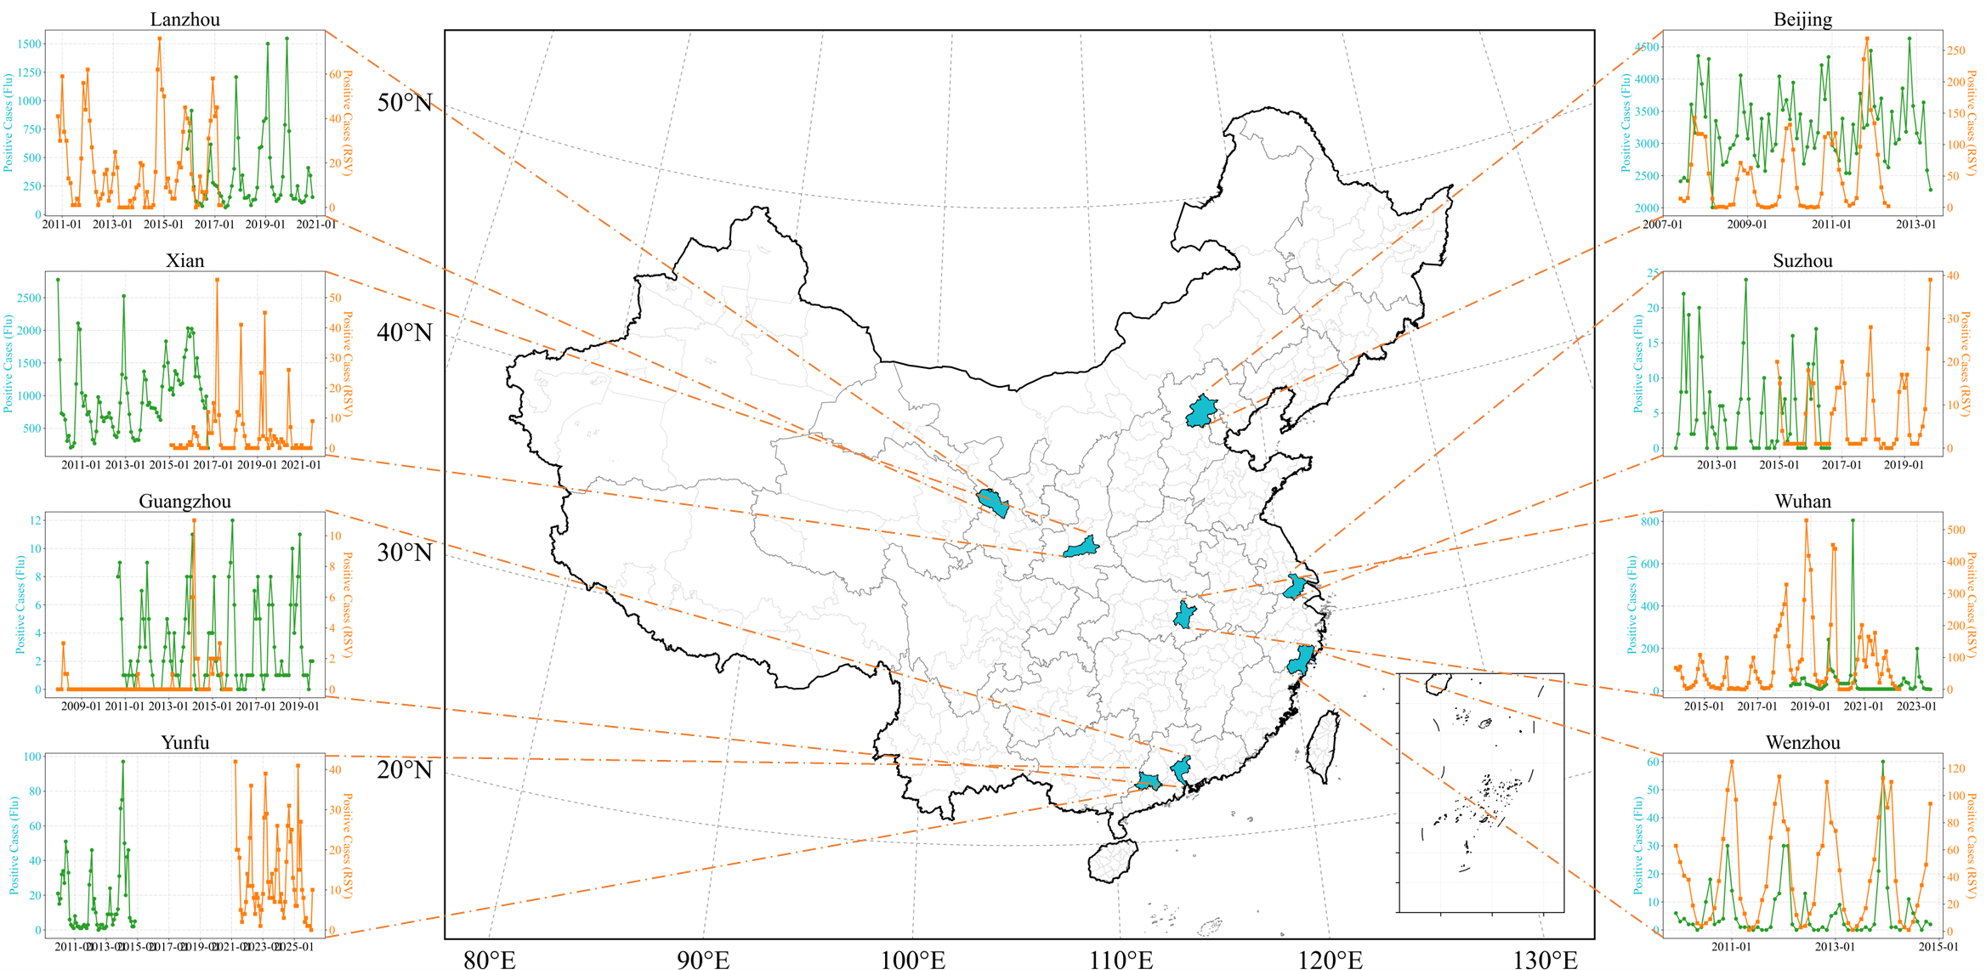
\includegraphics[width=0.8\textwidth]{../figures/Figure 1.png}
  \caption{The geographic location of the eight study cities across mainland China and the historical epicurves of their seasonal influenza (green) and RSV (orange) disease burden.}
  \label{fig:data_selection}
\end{figure}


\subsection{Identifying within- and between-year cycles}
% To enable comparison across cities and pathogens, all time series were normalised into dimensionless intensity indices after log-transformation.
% A small constant ($\epsilon = 10^{-6}$) was added to zero values prior to log-transformation to avoid undefined values.

We used a smoothing-based algorithm to extract the within- and between-year cycles from the disease burden time series for seasonal influenza and RSV. 
The foundation of this algorithm is LOESS (Locally Estimated Scatterplot Smoothing). 
Seasonal-Trend decomposition using LOESS (STL) is commonly used to extract within-year cycles in time-series data, assuming single internal cycles. 
The smoothing-based approach is numerically more flexible compared to other approaches that require researchers to make assumptions about expected mathematical forms (e.g. cosine models or cubic spline-based models) \cite{madaniyazi2022assessing}.  
We used STL to extract the within-year cycles from the disease burden time series for seasonal influenza and RSV as a baseline model.

We then used MSTL (Multiple Seasonal-Trend decomposition using LOESS), which allows for more than one cycle. 
With MSTL, the original time series were decomposed into four components: within-year patterns (also available through baseline STL models), between-year patterns, long-term trends, and residuals.
We assumed the within-year cycle lengths to be between 10 and 14 months and between-year cycle lengths to be between 18 and 36 months. 
The upper limit of the between-year cycle lengths was further constrained by the total lengths of the series. 
For time series that do not contain at least two full cycles of a given period length, MSTL does not test that between-year cycle length, as this is a requirement of the MSTL algorithm. 
In other words, for each city and pathogen combination, we tested up to 90 different model specifications (5 within-year cycle lengths * 18 between-year cycle lengths) using MSTL.
Correspondingly, we presented the STL comparator models using 5 different model specifications (5 within-year cycle lengths).

Model selection (from 5 STL models and up to 90 MSTL models) was performed using Akaike Information Criterion (AIC). 
The optimal model for each city-pathogen combination was defined as having the minimum AIC value. 
Following standard practice, we considered models with $\Delta$AIC $< 7$ (where $\Delta$AIC $= $ AIC$_i$ $-$ AIC$_{\text{min}}$) as having comparable empirical support. 
The optimal models and their comparable models were all included in further analysis (i.e. forward simulation and concurrent outbreak identification).
The lowest AIC estimates achievable using a single-cycle model (i.e. STL models) were compared against the lowest AIC estimates achievable using multi-cycle models (i.e. MSTL models) to assess whether the inclusion of a between-year cycle improves predictive performance.
If the latter is lower, then we conclude that between-year patterns contribute to predicting the burden in the context of the city-pathogen combination.
Bayesian Information Criterion (BIC) was also examined as a sensitivity analysis.

\subsection{Forward simulations of outbreaks and concurrent outbreak identification}
To assess the implications of within- and between-year patterns on future disease burden, we performed forward simulations based on observed disease burden history and the optimal and their comparable models derived using the methods above.
These forward simulations were performed for long timeframes to ensure that within- and between-year patterns estimated using different time series may be overlaid for a given city.
Within- and between-year patterns were simply repeated in these forward simulations.
The trend and residual component time series from the optimal STL/MSTL models were fitted using an Auto-Regressive Integrated Moving Average (ARIMA) model.
This ARIMA model was then used to generate 1000 stochastic forward trajectories of the trend and residual components per model selected.
Since the ARIMA model was fitted to a seasonally adjusted time series, the mean-reverting properties ensure that long-term forward simulations remain bounded.
This stochastic simulation framework was developed to characterise the uncertainty around event probabilities, rather than providing deterministic forecasts of future disease activities.
When a given city-pathogen combination has $n$ optimal models, then $1000 \times n$ stochastic forward trajectories were generated. 
All forward simulations were performed based on their original time scale, as presented in the source literature.

Using the forward simulations of both seasonal influenza and RSV disease burden, we explore the possibility of concurrent outbreaks across different outbreak thresholds. 
The measure of seasonal influenza and RSV disease burden relied on different epidemiological measures depending on the city and health systems (e.g. attributable hospital admissions, test positive rates) and therefore cannot be directly compared on their original scale.
Therefore, we rescaled these measures by decile, leaving the 1st and 10th deciles unbounded.
Concurrent outbreaks were defined to occur when seasonal influenza and RSV disease burden simultaneously exceeded the 70th, 80th, or 90th percentiles of their observed disease burden history.
A year is considered a concurrent outbreak year if the concurrent outbreak threshold was exceeded at least once in that year.

\subsection{Characterising concurrent outbreak frequency using survival analysis}
Inter-concurrent outbreak intervals were calculated as the time elapsed between successive concurrent outbreak years.
Directly counting the intervals between concurrent outbreaks over-weights short intervals as they have more placement opportunities given the finite forward simulation window.
It also introduces right-censoring issues when no concurrent outbreak or only one concurrent outbreak was observed in the forward simulation window.
To address these issues, we reframed the interval detection as a time-to-event problem, and estimated the inter-concurrent outbreak intervals using Kaplan-Meier survival analysis, with left truncation and right-censoring.
The survival curve was fitted for each city at all three different concurrent outbreak thresholds defined above.
With this setup, we can calculate inter-concurrent outbreak intervals.
In the context of this study, we used the time by which 50\% of the forward simulation paths ($1000 \times n$ models) are expected to experience their subsequent concurrent outbreak event as the inter-concurrent outbreak interval. 

\subsection{Software and code availability}
All aforementioned methods and analyses were implemented in R (v4.2.2) using the following \texttt{package}s: \texttt{forecast}, \texttt{mstl}, and \texttt{survival}. All codes are available on the GitHub repository: \url{https://github.com/yangclaraliu/respiratory_multi_pathogen_seasonality}.
